\section{Esperanza Condicionada}

\begin{ejercicio}
    Sea $X$ una variable aleatoria que se distribuye uniformemente en el intervalo $\left]0,1\right[$. Comprobar si las variables aleatorias $X$ y $|\nicefrac{1}{2}-X|$ son incorreladas.

    % // TODO: Incorreladas?
\end{ejercicio}

\begin{ejercicio}
    Calcular las curvas de regresión y las razones de correlación para las siguientes distribuciones, comentando los resultados.
    \begin{enumerate}
        \item Considerar las distribución conjunta $(X,Y)$ con función de masa de probabilidad dada por:
        \begin{equation*}
            \begin{array}{c|ccc||c}
                X\setminus Y & 10 & 15 & 20 & \\
                \hline
                1 & 0 & \nicefrac{2}{6} & 0 & \nicefrac{2}{6}\\
                2 & \nicefrac{1}{6} & 0 & 0 & \nicefrac{1}{6}\\
                3 & 0 & 0 & \nicefrac{3}{6} & \nicefrac{3}{6}\\
                \hline \hline
                & \nicefrac{1}{6} & \nicefrac{2}{6} & \nicefrac{3}{6} & 1
            \end{array}
        \end{equation*}

        Tras haber calculado las distribuciones marginales, calculamos ahora las distribuciones condicionadas.
        La siguiente tabla muestra la distribución condicionada de $Y$ dado $X$, $P[Y = y\mid X = x]$:
        \begin{equation*}
            \begin{array}{c|ccc}
                X\setminus Y & 10 & 15 & 20 \\
                \hline
                1 & 0 & 1 & 0\\
                2 & 1 & 0 & 0\\
                3 & 0 & 0 & 1
            \end{array}
        \end{equation*}

        La distribución condicionada de $X$ dado $Y$, $P[X = x\mid Y = y]$ viene dada por la misma tabla, ya que en este caso tenemos que:
        \begin{equation*}
            P[X = x\mid Y = y] = P[Y = y\mid X = x] \qquad \forall x, y
        \end{equation*}

        Calculemos ahora las curvas de regresión y las razones de correlación.
        \begin{itemize}
            \item Curva de regresión de $Y$ sobre $X$:
            \begin{equation*}
                \wh{Y}(x) = E[Y\mid X = x] = \sum_{y} y P[Y = y\mid X = x] \qquad \forall x\in E_x
            \end{equation*}
    
            Por tanto, la curva de regresión de $Y$ sobre $X$ es:
            \begin{equation*}
                \wh{Y}(1) = 15 \qquad \wh{Y}(2) = 10 \qquad \wh{Y}(3) = 20
            \end{equation*}

            Para calcular la razón de correlación de $Y$ sobre $X$,
            hay dos opciones:
            \begin{description}
                \item[Opción 1.] Método rutinario.
                
                Usamos la fórmula:
                \begin{equation*}
                    \eta^2_{Y/X} = \dfrac{\Var(E[Y\mid X])}{\Var(Y)}
                \end{equation*}
                \begin{itemize}
                    \item Calculemos $E[Y]$:
                    \begin{align*}
                        E[Y] &= \sum_{y} y P[Y = y]
                        &= 10 \cdot \nicefrac{1}{6} + 15 \cdot \nicefrac{2}{6} + 20 \cdot \nicefrac{3}{6}
                        = \frac{50}{3}
                    \end{align*}

                    \item Calculemos ahora $E[Y^2]$:
                    \begin{align*}
                        E[Y^2] &= \sum_{y} y^2 P[Y = y]
                        = 10^2 \cdot \nicefrac{1}{6} + 15^2 \cdot \nicefrac{2}{6} + 20^2 \cdot \nicefrac{3}{6}
                        = \frac{875}{3}
                    \end{align*}

                    \item Calculemos ahora $E[(E[Y\mid X])^2]$:
                    \begin{align*}
                        E[(E[Y\mid X])^2] &= \sum_{x} (E[Y\mid X = x])^2 P[X = x]
                        =\\&= 10^2 \cdot \nicefrac{1}{6} + 15^2 \cdot \nicefrac{2}{6} + 20^2 \cdot \nicefrac{3}{6}
                        = \frac{875}{3} = E[Y^2]
                    \end{align*}

                    \item Calculemos ahora $E[E[Y\mid X]]$.
                    \begin{equation*}
                        E[E[Y\mid X]] = E[Y]
                    \end{equation*}
                \end{itemize}

                Por tanto, usando lo anterior, tenemos:
                \begin{align*}
                    \eta^2_{Y/X} &= \dfrac{\Var(E[Y\mid X])}{\Var(Y)}
                    = \dfrac{E[(E[Y\mid X])^2] - E[E[Y\mid X]]^2}{E[Y^2] - E[Y]^2}\\
                    &= \dfrac{E[Y^2] - E[Y]^2}{E[Y^2] - E[Y]^2} = 1
                \end{align*}

                \item[Opción 2.] Razonando por dependencia funcional.
                
                En este caso, vemos que $Y$ es función de $X$. Por tanto:
                \begin{equation*}
                    \eta^2_{Y/X} = 1
                \end{equation*}
            \end{description}

            \item Curva de regresión de $X$ sobre $Y$:
            \begin{equation*}
                \wh{X}(y) = E[X\mid Y = y] = \sum_{x} x P[X = x\mid Y = y] \qquad \forall y\in E_y
            \end{equation*}

            Por tanto, la curva de regresión de $X$ sobre $Y$ es:
            \begin{equation*}
                \wh{X}(10) = 2 \qquad \wh{X}(15) = 1 \qquad \wh{X}(20) = 3
            \end{equation*}

            De nuevo, razonando ahora por dependencia funcional, tenemos que:
            \begin{equation*}
                \eta^2_{X/Y} = 1
            \end{equation*}
        \end{itemize}

        Como vemos, en este caso, hay dependencia recíproca entre $X$ e $Y$. Por tanto,
        el ajuste es el idea, ya que $Y=f(X)$ y $X=g(Y)$.
        Cada una explica la totalidad de la variabilidad de la otra.


        \item Considerar las distribución conjunta $(X,Y)$ con función de masa de probabilidad dada por:
        \begin{equation*}
            \begin{array}{c|cccc||c}
                X\setminus Y & 10 & 15 & 20 & 25 &\\
                \hline
                1 & 0 & \nicefrac{3}{7} & 0 & \nicefrac{1}{7} & \nicefrac{4}{7}\\
                2 & 0 & 0 & \nicefrac{1}{7} & 0 & \nicefrac{1}{7}\\
                3 & \nicefrac{2}{7} & 0 & 0 & 0 & \nicefrac{2}{7}\\
                \hline \hline
                & \nicefrac{2}{7} & \nicefrac{3}{7} & \nicefrac{1}{7} & \nicefrac{1}{7} & 1
            \end{array}
        \end{equation*}

        Tras haber calculado las distribuciones marginales, calculamos ahora las distribuciones condicionadas.
        La siguiente tabla muestra la distribución condicionada de $Y$ dado $X$, $P[Y = y\mid X = x]$:
        \begin{equation*}
            \begin{array}{c|cccc}
                X\setminus Y & 10 & 15 & 20 & 25\\
                \hline
                1 & 0 & \nicefrac{3}{4} & 0 & \nicefrac{1}{4}\\
                2 & 0 & 0 & 1 & 0\\
                3 & 1 & 0 & 0 & 0
            \end{array}
        \end{equation*}

        La distribución condicionada de $X$ dado $Y$, $P[X = x\mid Y = y]$ viene dada por la siguiente tabla:
        \begin{equation*}
            \begin{array}{c|ccc}
                X\setminus Y & 10 & 15 & 20\\
                \hline
                1 & 0 & 1 & 0\\
                2 & 0 & 0 & 1\\
                3 & 1 & 0 & 0
            \end{array}
        \end{equation*}

        Calculemos ahora las curvas de regresión y las razones de correlación.
        \begin{itemize}
            \item Curva de regresión de $Y$ sobre $X$:
            \begin{equation*}
                \wh{Y}(x) = E[Y\mid X = x] = \sum_{y} y P[Y = y\mid X = x] \qquad \forall x\in E_x
            \end{equation*}

            Por tanto, la curva de regresión de $Y$ sobre $X$ es:
            \begin{align*}
                \wh{Y}(1) &= 15\cdot \nicefrac{3}{4} + 25\cdot \nicefrac{1}{4} = 17.5\\
                \wh{Y}(2) &= 20\\
                \wh{Y}(3) &= 10
            \end{align*}

            Para calcular la razón de correlación de $Y$ sobre $X$, tenemos que:
            \begin{equation*}
                \eta^2_{Y/X} = \dfrac{\Var(E[Y\mid X])}{\Var(Y)}
            \end{equation*}
            \begin{itemize}
                \item Calculemos $E[Y]$:
                \begin{align*}
                    E[Y] &= \sum_{y} y P[Y = y]
                    = 10 \cdot \nicefrac{2}{7} + 15 \cdot \nicefrac{3}{7} + 20 \cdot \nicefrac{1}{7} + 25 \cdot \nicefrac{1}{7}
                    = \frac{110}{7}
                \end{align*}

                \item Calculemos ahora $E[Y^2]$:
                \begin{align*}
                    E[Y^2] &= \sum_{y} y^2 P[Y = y]\\
                    &= 10^2 \cdot \nicefrac{2}{7} + 15^2 \cdot \nicefrac{3}{7} + 20^2 \cdot \nicefrac{1}{7} + 25^2 \cdot \nicefrac{1}{7}
                    = \frac{1900}{7}
                \end{align*}

                \item Calculemos ahora $E[(E[Y\mid X])^2]$:
                \begin{align*}
                    E[(E[Y\mid X])^2] &= \sum_{x} (E[Y\mid X = x])^2 P[X = x]\\
                    &= 17.5^2 \cdot \nicefrac{4}{7} + 20^2 \cdot \nicefrac{1}{7} + 10^2 \cdot \nicefrac{2}{7}
                    = \frac{1825}{7}
                \end{align*}

                \item Calculemos ahora $E[E[Y\mid X]]$.
                \begin{equation*}
                    E[E[Y\mid X]] = E[Y]
                \end{equation*}
            \end{itemize}

            Por tanto, usando lo anterior, tenemos:
            \begin{align*}
                \eta^2_{Y/X} &= \dfrac{\Var(E[Y\mid X])}{\Var(Y)}
                = \dfrac{E[(E[Y\mid X])^2] - E[E[Y\mid X]]^2}{E[Y^2] - E[Y]^2}\\
                &= \dfrac{E[(E[Y\mid X])^2] - E[Y]^2}{E[Y^2] - E[Y]^2}\\
                &= \dfrac{\dfrac{1825}{7} - \left(\dfrac{110}{7}\right)^2}{\dfrac{1900}{7} - \left(\dfrac{110}{7}\right)^2}
                = \dfrac{9}{16} \approx 0.5625
            \end{align*}

            Por tanto, tenemos que $X$ explica el $56.25\%$ de la variabilidad de $Y$. Tenemos entonces que no es un ajuste ideal.

            \item Curva de regresión de $X$ sobre $Y$:
            
            En este caso, tenemos que $X=f(Y)$, por lo que:
            \begin{equation*}
                \wh{X}(10) = 3, \quad \wh{X}(15) = 1, \quad \wh{X}(20) = 2, \quad \wh{X}(25) = 1
            \end{equation*}

            Por tanto, como $X$ es función de $Y$, tenemos que:
            \begin{equation*}
                \eta^2_{X/Y} = 1
            \end{equation*}

            Tenemos que $Y$ explica la totalidad de la variabilidad de $X$, por lo que el ajuste es el ideal.
        \end{itemize}


    \end{enumerate}
\end{ejercicio}

\begin{ejercicio}
    Sea $X$ el número de balanzas e $Y$ el número de dependientes en los puntos de venta de un mercado. Determinar las rectas de regresión y el grado de ajuste a la distribución, si la función masa de probabilidad de $(X,Y)$ viene dada por:
    \begin{equation*}
        \begin{array}{c|cccc||c}
            X\setminus Y & 1 & 2 & 3 & 4\\
            \hline
            1 & \nicefrac{1}{24} & \nicefrac{2}{24} & 0 & 0 & \nicefrac{3}{24}\\
            2 & \nicefrac{1}{24} & \nicefrac{2}{24} & \nicefrac{3}{24} & \nicefrac{1}{24} & \nicefrac{7}{24}\\
            3 & 0 & \nicefrac{1}{24} & \nicefrac{2}{24} & \nicefrac{6}{24} & \nicefrac{9}{24}\\
            4 & 0 & 0 & \nicefrac{2}{24} & \nicefrac{3}{24} & \nicefrac{5}{24}\\
            \hline \hline
            & \nicefrac{2}{24} & \nicefrac{5}{24} & \nicefrac{7}{24} & \nicefrac{10}{24} & 1
        \end{array}
    \end{equation*}

    Tras calcular las distribuciones marginales, calculamos ahora las esperanzas necesarias para que el resto de cálculos posteriormente sean directos.
    \begin{align*}
        E[X] &= 1\cdot \nicefrac{3}{24} + 2\cdot \nicefrac{7}{24} + 3\cdot \nicefrac{9}{24} + 4\cdot \nicefrac{5}{24} = \nicefrac{8}{3}\\
        E[Y] &= 1\cdot \nicefrac{2}{24} + 2\cdot \nicefrac{5}{24} + 3\cdot \nicefrac{7}{24} + 4\cdot \nicefrac{10}{24} = \nicefrac{73}{24}\\
        E[X^2] &= 1^2\cdot \nicefrac{3}{24} + 2^2\cdot \nicefrac{7}{24} + 3^2\cdot \nicefrac{9}{24} + 4^2\cdot \nicefrac{5}{24} = 8\\
        E[Y^2] &= 1^2\cdot \nicefrac{2}{24} + 2^2\cdot \nicefrac{5}{24} + 3^2\cdot \nicefrac{7}{24} + 4^2\cdot \nicefrac{10}{24} = \nicefrac{245}{24}\\
        E[XY] &= \sum_{\substack{x\in E_X\\y\in E_y}}xyP[X = x, Y = y] = \nicefrac{209}{24}\\
        \Var[X] &= E[X^2] - E[X]^2 = \nicefrac{8}{9}\\
        \Var[Y] &= E[Y^2] - E[Y]^2 = \nicefrac{551}{576}\\
        \Cov[X,Y] &= E[XY] - E[X]E[Y] = \nicefrac{43}{72}
    \end{align*}

    Calculamos ahora las rectas de regresión.
    \begin{itemize}
        \item Recta de regresión de $Y$ sobre $X$:
        \begin{align*}
            \wh{Y}(x) &= E[Y] + \dfrac{\Cov[X,Y]}{\Var[X]}(X - E[X])
            = \frac{73}{24} + \dfrac{\nicefrac{43}{72}}{\nicefrac{8}{9}}(X - \nicefrac{8}{3})
            =\\&= \nicefrac{73}{24} + \dfrac{43}{64}(X - \nicefrac{8}{3})
        \end{align*}

        \item Recta de regresión de $X$ sobre $Y$:
        \begin{align*}
            \wh{X}(y) &= E[X] + \dfrac{\Cov[X,Y]}{\Var[Y]}(Y - E[Y])
            = \nicefrac{8}{3} + \dfrac{\nicefrac{43}{72}}{\nicefrac{551}{576}}(Y - \nicefrac{73}{24})
            =\\&= \nicefrac{8}{3} + \dfrac{344}{551}(Y - \nicefrac{73}{24})
        \end{align*}
    \end{itemize}

    Para determinar el grado de ajuste a la distribución, calculamos ahora el coeficiente de determinación lineal:
    \begin{equation*}
        \rho_{Y/X}^2 = \dfrac{\Cov[X,Y]^2}{\Var[X]\Var[Y]} = \dfrac{1849}{4408} \approx 0.419
    \end{equation*}

    Por tanto, tenemos que el $41.9\%$ de la variabilidad de $Y$ queda explicada por la regresión lineal de $Y$ sobre $X$.
    Vemos por tanto que el ajusto no es bueno.
\end{ejercicio}

\begin{ejercicio}
    Sea $(X,Y)$ un vector aleatorio con valores en el conjunto dado por $T=\{(x, y) \in \mathbb{R}^2/0 < x < y < 2\}$ y función de densidad constante. Calcular:
    \begin{enumerate}
        \item Función de densidad de probabilidad conjunta.
        
        Veamos en primer lugar el conjunto en el que se distribuye el vector aleatorio $(X,Y)$:
        \begin{figure}[H]
            \centering
            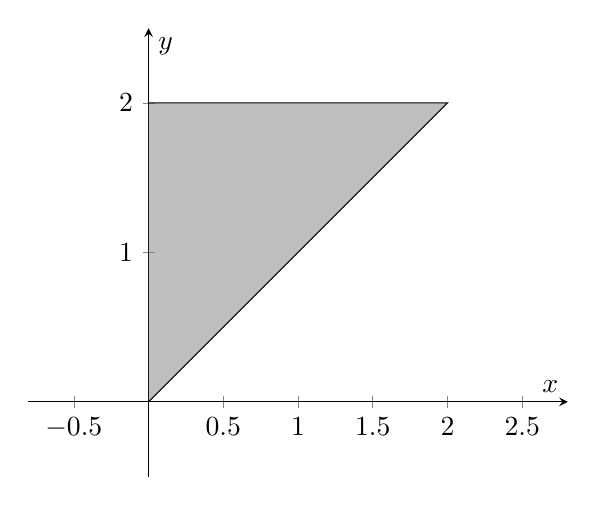
\begin{tikzpicture}
                \begin{axis}[
                    axis lines = center,
                    xlabel = $x$,
                    ylabel = $y$,
                    xmin = -0.5, xmax = 2.5,
                    ymin = -0.5, ymax = 2.5,
                    legend pos = north west,
                    axis equal,
                ]
                    % Triángulo (0,0) (2,2) (0,2)
                    \addplot[fill=gray, fill opacity=0.5] coordinates {(0,0) (2,2) (0,2)};
                \end{axis}
            \end{tikzpicture}
        \end{figure}

        Como la función de densidad es constante, tenemos que:
        \begin{equation*}
            f_{(X,Y)}(x, y) = \begin{cases}
                k, & (x, y) \in T \\
                0, & \text{en otro caso}
            \end{cases}
        \end{equation*}

        Para calcular $k$, tenemos que:
        \begin{align*}
            1 &= \int_{T} f_{(X,Y)} = \int_T k = k\lm(T) = k\cdot 2
            \Longrightarrow k=\nicefrac{1}{2}
        \end{align*}
        \item Curvas y rectas de regresión de $X$ sobre $Y$ y de $Y$ sobre $X$.
        
        Comenzamos calculando las curvas de regresión, ya que si estas son funciones lineales, las rectas de regresión coincidirán con las curvas de regresión.
        Para ello, calculamos las funciones de densidad marginales y condicionadas.
        \begin{itemize}
            \item Función de densidad de $X$. Para $x\in \left]0,2\right[$:
            \begin{align*}
                f_X(x) &= \int_{-\infty}^{\infty} f_{(X,Y)}(x, y) \ dy
                = \int_{x}^{2} \nicefrac{1}{2} \ dy = \nicefrac{1}{2}(2-x)
                = 1-\frac{x}{2}
            \end{align*}

            \item Función de densidad de $Y$. Para $y\in \left]0,2\right[$:
            \begin{align*}
                f_Y(y) &= \int_{-\infty}^{\infty} f_{(X,Y)}(x, y) \ dx
                = \int_{0}^{y} \nicefrac{1}{2} \ dx = \frac{y}{2}
            \end{align*}

            \item Función de densidad condicionada de $X$ dado $Y=y^*\in \left]0,2\right[$. Para $x\in \left]0,y^*\right[$:
            \begin{align*}
                f_{X\mid Y=y^*}(x) &= \dfrac{f_{(X,Y)}(x, y^*)}{f_Y(y^*)}
                = \dfrac{\nicefrac{1}{2}}{\nicefrac{y^*}{2}}
                = \dfrac{1}{y^*}
            \end{align*}

            \item Función de densidad condicionada de $Y$ dado $X=x^*\in \left]0,2\right[$. Para $y\in \left]x^*,2\right[$:
            \begin{align*}
                f_{Y\mid X=x^*}(y) &= \dfrac{f_{(X,Y)}(x^*, y)}{f_X(x^*)}
                = \dfrac{\nicefrac{1}{2}}{1-\nicefrac{x^*}{2}}
                = \dfrac{1}{2-x^*}
            \end{align*}
        \end{itemize}

        Calculamos ahora las curvas de regresión.
        \begin{itemize}
            \item Curva de regresión de $X$ sobre $Y$:
            \begin{align*}
                \wh{X}(y) &= E[X\mid Y = y] = \int_{0}^{y} x f_{X\mid Y=y}(x) \ dx
                = \int_{0}^{y} x\cdot  \dfrac{1}{y} \ dx
                = \dfrac{1}{y} \int_{0}^{y} x \ dx
                =\\&= \dfrac{1}{y} \left[\dfrac{x^2}{2}\right]_{0}^{y}
                = \dfrac{y}{2} \qquad \forall y\in \left]0,2\right[
            \end{align*}

            \item Curva de regresión de $Y$ sobre $X$:
            \begin{align*}
                \wh{Y}(x) &= E[Y\mid X = x] = \int_{x}^{2} y f_{Y\mid X=x}(y) \ dy
                = \int_{x}^{2} y\cdot  \dfrac{1}{2-x} \ dy
                = \dfrac{1}{2-x} \int_{x}^{2} y \ dy
                =\\&= \dfrac{1}{2-x} \left[\dfrac{y^2}{2}\right]_{x}^{2}
                = \dfrac{2^2 - x^2}{2(2-x)}
                = \dfrac{4-x^2}{2(2-x)}
                = \dfrac{2+x}{2} = 1 + \dfrac{x}{2} \qquad \forall x\in \left]0,2\right[
            \end{align*}
        \end{itemize}

        Tenemos además que las curvas de regresión son funciones lineales, por lo que las rectas de regresión coinciden con las curvas de regresión.
        \item Razones de correlación y coeficiente de correlación lineal.
        
        Como las curvas de regresión son funciones lineales, tenemos que las razones de correlación coinciden y son iguales al coeficiente de determinación lineal.
        \begin{equation*}
            \eta_{Y/X}^2 = \eta_{X/Y}^2 = \rho_{Y/X}^2 = \dfrac{\Cov[X,Y]^2}{\Var[X]\Var[Y]}
        \end{equation*}
        
        Como este es el producto de las pendientes de las rectas de regresión, tenemos que:
        \begin{equation*}
            \rho_{Y/X}^2 = \dfrac{1}{2}\cdot \dfrac{1}{2} = \dfrac{1}{4}
        \end{equation*}

        Como la correlación es positiva por ser ambas rectas crecientes, tenemos que:
        \begin{equation*}
            \rho_{Y/X} =  + \sqrt{\rho_{Y/X}^2} = \nicefrac{1}{2}
        \end{equation*}

        \item Error cuadrático medio asociado a cada una de las funciones de regresión.
        
        Por lo visto en teoría, sabemos que:
        \begin{align*}
            \text{ECM}(\wh{X}) &= \Var[X] - \dfrac{\Cov[X,Y]^2}{\Var[Y]}\\
            \text{ECM}(\wh{Y}) &= \Var[Y] - \dfrac{\Cov[X,Y]^2}{\Var[X]}
        \end{align*}

        Calculamos por tanto los valores necesarios:
        \begin{align*}
            E[X] &= \int_{0}^{2} x f_X(x) \ dx = \int_{0}^{2} x(1-\nicefrac{x}{2}) \ dx
            = \left[\dfrac{x^2}{2} - \dfrac{x^3}{6}\right]_{0}^{2}
            = \dfrac{4}{2} - \dfrac{8}{6} = \dfrac{2}{3}\\
            E[Y] &= \int_{0}^{2} y f_Y(y) \ dy = \int_{0}^{2} y\cdot \nicefrac{y}{2} \ dy
            = \left[\dfrac{y^3}{6}\right]_{0}^{2} = \dfrac{8}{6} = \frac{4}{3}\\
            E[X^2] &= \int_{0}^{2} x^2 f_X(x) \ dx = \int_{0}^{2} x^2(1-\nicefrac{x}{2}) \ dx
            = \left[\dfrac{x^3}{3} - \dfrac{x^4}{8}\right]_{0}^{2}
            = \dfrac{8}{3} - \dfrac{16}{8} = \dfrac{2}{3}\\
            E[Y^2] &= \int_{0}^{2} y^2 f_Y(y) \ dy = \int_{0}^{2} y^2\cdot \nicefrac{y}{2} \ dy
            = \left[\dfrac{y^4}{8}\right]_{0}^{2} = \dfrac{16}{8} = 2\\
            E[XY] &= \int_{0}^{2} \int_{x}^{2} xy f_{(X,Y)}(x, y) \ dy \ dx
            = \int_{0}^{2} \int_{x}^{2} xy\cdot \nicefrac{1}{2} \ dy \ dx
            = \frac{1}{2} \int_{0}^{2} x\left[\dfrac{y^2}{2}\right]_{x}^{2} \ dx
            =\\&= \frac{1}{4} \int_{0}^{2} x\left(4 - x^2\right) \ dx
            = \frac{1}{4} \left[2x^2 - \frac{x^4}{4}\right]_{0}^{2}
            = \frac{1}{4} \left(8 - 4\right) = 1\\
            \Var[X] &= E[X^2] - E[X]^2 = \frac{2}{3} - \left(\frac{2}{3}\right)^2 = \frac{2}{9}\\
            \Var[Y] &= E[Y^2] - E[Y]^2 = 2 - \left(\frac{4}{3}\right)^2 = \frac{2}{9}\\
            \Cov[X,Y] &= E[XY] - E[X]E[Y] = 1 - \frac{2}{3}\cdot \frac{4}{3} = \frac{1}{9}
        \end{align*}

        Por tanto, tenemos que:
        \begin{align*}
            \text{ECM}(\wh{X}) &= \Var[X] - \dfrac{\Cov[X,Y]^2}{\Var[Y]}
            = \frac{2}{9} - \dfrac{\nicefrac{1}{9}^2}{\nicefrac{2}{9}}
            = \frac{2}{9} - \frac{1}{18} = \frac{3}{18} = \frac{1}{6}\\
            \text{ECM}(\wh{Y}) &= \Var[Y] - \dfrac{\Cov[X,Y]^2}{\Var[X]}
            = \frac{2}{9} - \dfrac{\nicefrac{1}{9}^2}{\nicefrac{2}{9}}
            = \frac{2}{9} - \frac{1}{18} = \frac{3}{18} = \frac{1}{6}
        \end{align*}
    \end{enumerate}
\end{ejercicio}

\begin{ejercicio}
    Dada la función masa de probabilidad del vector aleatorio $(X,Y)$
    \begin{equation*}
        \begin{array}{c|cccc||c}
            X\setminus Y & 0 & 1 & 2 & 3\\
            \hline
            0 & 0.2 & 0.2 & 0.05 & 0 & 0.45\\
            1 & 0.1 & 0.1 & 0.1 & 0.05 & 0.35\\
            2 & 0 & 0.05 & 0.05 & 0.1 & 0.2\\
            \hline \hline
            & 0.3 & 0.35 & 0.2 & 0.15 & 1
        \end{array}
    \end{equation*}
    \begin{enumerate}
        \item Determinar la aproximación lineal mínimo cuadrática de $Y$ para $X = 1$.
        
        Nos piden la recta de regresión de $Y$ sobre $X$, y evaluarla en el punto $X=1$.
        Calculamos las esperanzas necesarias para el cálculo de la recta de regresión.
        \begin{align*}
            E[X] &= 0\cdot 0.3 + 1\cdot 0.35 + 2\cdot 0.2 = 0.75\\
            E[Y] &= 0\cdot 0.3 + 1\cdot 0.35 + 2\cdot 0.2 + 3\cdot 0.15 = 1.2\\
            E[X^2] &= 0^2\cdot 0.3 + 1^2\cdot 0.35 + 2^2\cdot 0.2 = 1.15\\
            E[XY] &= \sum_{\substack{x\in E_X\\y\in E_Y}}xyP[X = x, Y = y] = 1.35\\
            \Var[X] &= E[X^2] - E[X]^2 = 1.15 - 0.75^2 = 0.5875\\
            \Cov[X,Y] &= E[XY] - E[X]E[Y] = 1.35 - 0.75\cdot 1.2 = 0.45
        \end{align*}

        Calculamos ahora la recta de regresión de $Y$ sobre $X$.
        \begin{align*}
            \wh{Y}(x) &= E[Y] + \dfrac{\Cov[X,Y]}{\Var[X]}(x - E[X])
            = 1.2 + \dfrac{0.45}{0.5875}(x - 0.75)
            = 1.2 + \dfrac{36}{47}(x - 0.75)
        \end{align*}

        Evaluando en $X=1$, tenemos que:
        \begin{equation*}
            \wh{Y}(1) = 1.2 + \dfrac{36}{47}(1 - 0.75) = 1.2 + \dfrac{36}{47}\cdot 0.25 = 1.2 + \dfrac{9}{47} \approx 1.391489
        \end{equation*}
        \item Determinar la aproximación mínimo cuadrática de $Y$ para $X = 1$.
        
        En este caso, piden $E[Y\mid X = 1]$. Para ello, hemos de calcular las distribución condicionada de $Y$ dado $X = 1$.
        \begin{align*}
            P[Y = 0\mid X = 1] &= \dfrac{P[X = 1, Y = 0]}{P[X = 1]} = \dfrac{0.1}{0.35} = \frac{2}{7}\\
            P[Y = 1\mid X = 1] &= \dfrac{P[X = 1, Y = 1]}{P[X = 1]} = \dfrac{0.1}{0.35} = \frac{2}{7}\\
            P[Y = 2\mid X = 1] &= \dfrac{P[X = 1, Y = 2]}{P[X = 1]} = \dfrac{0.1}{0.35} = \frac{2}{7}\\
            P[Y = 3\mid X = 1] &= \dfrac{P[X = 1, Y = 3]}{P[X = 1]} = \dfrac{0.05}{0.35} = \frac{1}{7}
        \end{align*}

        Por tanto, tenemos que:
        \begin{align*}
            E[Y\mid X = 1] &= \sum_{y\in E_Y} y P[Y = y\mid X = 1] =\\&= 0+1\cdot P[Y = 1\mid X = 1] + 2\cdot P[Y = 2\mid X = 1] + 3\cdot P[Y = 3\mid X = 1]
            =\\&= \dfrac{2}{7} + 2\cdot \dfrac{2}{7} + 3\cdot \dfrac{1}{7} = \dfrac{9}{7}
        \end{align*}
    \end{enumerate}
\end{ejercicio}

\begin{ejercicio}
    Dadas las siguientes distribuciones, determinar qué variable, $X$ ó $X'$, aproxima mejor a la variable $Y$:
    \begin{equation*}
        \begin{array}{c|ccc||c}
            X\setminus Y & 0 & 1 & 2\\
            \hline
            0 & \nicefrac{1}{5} & 0 & 0 & \nicefrac{1}{5}\\
            2 & 0 & \nicefrac{1}{5} & 0 & \nicefrac{1}{5}\\
            3 & \nicefrac{1}{5} & 0 & \nicefrac{1}{5} & \nicefrac{2}{5}\\
            4 & 0 & 0 & \nicefrac{1}{5} & \nicefrac{1}{5}\\
            \hline \hline
            & \nicefrac{2}{5} & \nicefrac{1}{5} & \nicefrac{2}{5} & 1
        \end{array}
        \hspace{2cm}
        \begin{array}{c|ccc||c}
            X'\setminus Y & 0 & 1 & 2\\
            \hline
            0 & \nicefrac{1}{5} & 0 & \nicefrac{1}{5} & \nicefrac{2}{5}\\
            2 & 0 & \nicefrac{1}{5} & 0 & \nicefrac{1}{5}\\
            3 & \nicefrac{1}{5} & 0 & 0 & \nicefrac{1}{5}\\
            4 & 0 & 0 & \nicefrac{1}{5} & \nicefrac{1}{5}\\
            \hline \hline
            & \nicefrac{2}{5} & \nicefrac{1}{5} & \nicefrac{2}{5} & 1
        \end{array}
    \end{equation*}

    Hemos de obtener $\eta^2_{Y/X}$ y $\eta^2_{Y/X'}$ para compararlas.
    \begin{equation*}
        \eta^2_{Y/X} = \dfrac{\Var[E[Y\mid X]]}{\Var[Y]}, \qquad \eta^2_{Y/X'} = \dfrac{\Var[E[Y\mid X']]}{\Var[Y]}
    \end{equation*}

    Calculamos las esperanzas necesarias para el cálculo de las varianzas.
    \begin{align*}
        E[Y] &= 0\cdot \nicefrac{2}{5} + 1\cdot \nicefrac{1}{5} + 2\cdot \nicefrac{2}{5} = 1\\
        E[Y^2] &= 0^2\cdot \nicefrac{2}{5} + 1^2\cdot \nicefrac{1}{5} + 2^2\cdot \nicefrac{2}{5} = \nicefrac{9}{5}\\
        E[E[Y\mid X]] &= E[Y] = 1\\
        E[E[Y\mid X']] &= E[Y] = 1 \\
        E[(E[Y\mid X])^2] &= \sum_{x\in E_X} (E[Y\mid X = x])^2 P[X = x]\\
        E[(E[Y\mid X'])^2] &= \sum_{x\in E_{X'}} (E[Y\mid X' = x])^2 P[X' = x]
    \end{align*}

    Calculamos por tanto las esperanzas condicionadas.
    \begin{align*}
        E[Y\mid X = 0] &= 0\cdot 1 + 1\cdot 0 + 2\cdot 0 = 0\\
        E[Y\mid X = 2] &= 0\cdot 0 + 1\cdot 1 + 2\cdot 0 = 1\\
        E[Y\mid X = 3] &= 0\cdot \nicefrac{1}{2} + 1\cdot 0 + 2\cdot \nicefrac{1}{2} = 1\\
        E[Y\mid X = 4] &= 0\cdot 0 + 1\cdot 0 + 2\cdot 1 = 2\\
        E[Y\mid X' = 0] &= 0\cdot \nicefrac{1}{2} + 1\cdot 0 + 2\cdot \nicefrac{1}{2} = 1\\
        E[Y\mid X' = 2] &= 0\cdot 0 + 1\cdot 1 + 2\cdot 0 = 1\\
        E[Y\mid X' = 3] &= 0\cdot \nicefrac{1}{2} + 1\cdot 0 + 2\cdot \nicefrac{1}{2} = 1\\
        E[Y\mid X' = 4] &= 0\cdot 0 + 1\cdot 0 + 2\cdot 1 = 2
    \end{align*}

    Por tanto, hemos comprobado que $E[Y\mid X] = E[Y\mid X']$, por lo que:
    \begin{equation*}
        E[Y\mid X]=E[Y\mid X'] \Longrightarrow
        \Var[E[Y\mid X]] = \Var[E[Y\mid X']]
        \Longrightarrow \eta^2_{Y/X} = \eta^2_{Y/X'}
    \end{equation*}

    Por tanto, ambas variables aproximan igual de bien a $Y$. Veamos cómo es la aproximación calculando aun así los coeficientes. Tenemos que:
    \begin{align*}
        E[(E[Y\mid X])^2] &= \sum_{x\in E_X} (E[Y\mid X = x])^2 P[X = x]
        =\\&= 0^2\cdot \nicefrac{1}{5} + 1^2\cdot \nicefrac{1}{5} + 1^2\cdot \nicefrac{2}{5} + 2^2\cdot \nicefrac{1}{5} = \nicefrac{7}{5}
    \end{align*}

    Por tanto, tenemos que:
    \begin{align*}
        \Var[Y] = E[Y^2] - E[Y]^2 = \nicefrac{9}{5} - 1 = \nicefrac{4}{5}\\
        \Var[E[Y\mid X]] = E[(E[Y\mid X])^2] - E[E[Y\mid X]]^2 = \nicefrac{7}{5} - 1 = \nicefrac{2}{5}
    \end{align*}

    Por tanto, tenemos que:
    \begin{equation*}
        \eta^2_{Y/X} = \dfrac{\Var[E[Y\mid X]]}{\Var[Y]} = \dfrac{\nicefrac{2}{5}}{\nicefrac{4}{5}} = \nicefrac{1}{2} = \eta^2_{Y/X'}
    \end{equation*}

    Por tanto, tenemos que ninguno de los ajustes es bueno, ya que solo explican la mitad de la variabilidad de $Y$.
\end{ejercicio}

\begin{ejercicio} \label{ej:4.7}
    Probar que las variables $X = U + V$ e $Y = U - V$ son incorreladas, pero no independientes, si $U$ y $V$ son variables aleatorias con función de densidad conjunta:
    \begin{equation*}
        f_{U,V}(u, v) = \exp(-u-v), \quad u, v > 0.
    \end{equation*}

    % // TODO: Incorreladas?
    % Es la forma más fácil

    Veamos que no son independientes. Para ello, calculamos en primer lugar $f_{X,Y}(x, y)$. Para ello, definimos la transformación:
    \Func{g}{\mathbb{R}^2}{\mathbb{R}^2}{(U,V)}{(X,Y)=(U+V,U-V)}

    Para obtener $g^{-1}$, buscamos obtener $U,V$ en función de $X,T$:
    \begin{equation*}
        \left\{
            \begin{aligned}
                X=U+V\\
                Y=U-V
            \end{aligned}
        \right\}
        \Longrightarrow
        \left\{
            \begin{aligned}
                U=\nicefrac{X+Y}{2}\\
                V=\nicefrac{X-Y}{2}
            \end{aligned}
        \right\}
    \end{equation*}

    Por tanto, tenemos que $\exists g^{-1}$, con:
    \Func{g^{-1}}{\mathbb{R}^2}{\mathbb{R}^2}{(X,Y)}{(U,V)=\left(\frac{X+Y}{2},\frac{X-Y}{2}\right)}

    Tenemos que todas las componentes de $g^{-1}$ son derivables:
    \begin{align*}
        \dfrac{\partial U}{\partial X} &= \dfrac{1}{2}, & \dfrac{\partial U}{\partial Y} &= \dfrac{1}{2}, & \dfrac{\partial V}{\partial X} &= \dfrac{1}{2}, & \dfrac{\partial V}{\partial Y} &= -\dfrac{1}{2}
    \end{align*}

    Además, veamos que el jacobianos no se anula:
    \begin{equation*}
        \det Jg^{-1}(x,y)=\begin{vmatrix}
            \nicefrac{1}{2} & \nicefrac{1}{2}\\
            \nicefrac{1}{2} & \nicefrac{-1}{2}
        \end{vmatrix}=
        \dfrac{1}{2^2}\cdot \begin{vmatrix}
            1 & 1\\
            1 & -1
        \end{vmatrix}=
        -\frac{1}{2}\neq 0 \qquad \forall (x,y)\in\bb{R}^2.
    \end{equation*}

    Por tanto, podemos aplicar el teorema del cambio de variable para obtener $f_{X,Y}(x,y)$:
    \begin{align*}
        f_{X,Y}(x,y) &= f_{U,V}(g^{-1}(x,y))\cdot |Jg^{-1}(x,y)|
        = \dfrac{1}{2}\cdot f_{U,V}\left(\frac{x+y}{2},\frac{x-y}{2}\right)\\
        &= \dfrac{1}{2}\cdot \exp\left(-\frac{x+y}{2}-\frac{x-y}{2}\right)
        = \dfrac{1}{2}\cdot \exp\left(\dfrac{-x-y-x+y}{2}\right)
        =\\&= \dfrac{1}{2}\cdot \exp\left(-x\right)
        \qquad \forall (x,y)\in \bb{R}^2 \text{ tal que } x+y, x-y>0
    \end{align*}

    Veamos el conjunto gráficamente:
    \begin{figure}[H]
        \centering
        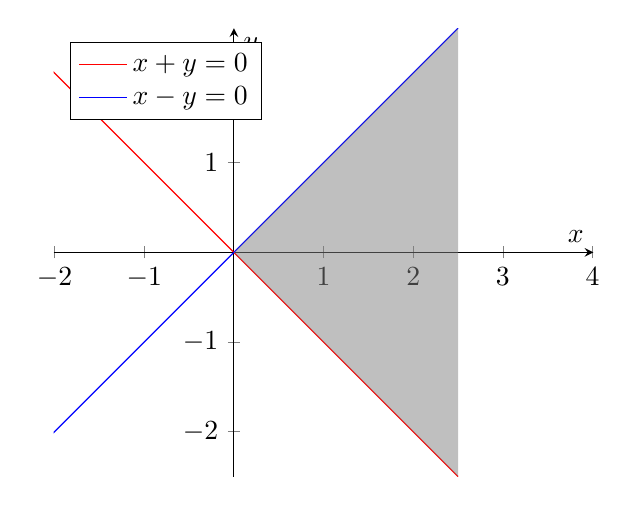
\begin{tikzpicture}
            \begin{axis}[
                axis lines = center,
                xlabel = $x$,
                ylabel = $y$,
                xmin = -0.5, xmax = 2.5,
                ymin = -2.5, ymax = 2.5,
                legend pos = north west,
                axis equal,
            ]
                % Recta x+y=0
                \addplot[domain=-5:2.5, samples=2, color=red]{-x};
                \addlegendentry{$x+y=0$}

                % Recta x-y=0
                \addplot[domain=-5:2.5, samples=2, color=blue]{x};
                \addlegendentry{$x-y=0$}

                % triangulo (0,0) (5,5) (5,-5)
                \addplot[fill=gray, fill opacity=0.5, draw=none] coordinates {(0,0) (2.5,2.5) (2.5,-2.5)};
            \end{axis}
        \end{tikzpicture}
    \end{figure}

    Tenemos que el conjunto donde $f_{X,Y}(x,y)$ no se puede expresar como producto cartesiano, por lo que intuimos que $X$ e $Y$ no son independientes. Para comprobarlo, calculamos la función de densidad marginal de $X$ y $Y$:
    \begin{align*}
        f_X(x) &= \int_{-\infty}^{\infty} f_{X,Y}(x, y) \ dy
        = \int_{-x}^{x} \nicefrac{1}{2}\exp(-x) \ dy
        = \nicefrac{1}{2}\exp(-x)\left[y\right]_{-x}^{x}
        =\\&= \nicefrac{1}{2}\exp(-x)(x+x) = xe^{-x} \qquad \forall x>0
    \end{align*}

    Para calcular la marginal de $Y$, distinguimos en función de $y$:
    \begin{itemize}
        \item Si $y>0$:
        \begin{align*}
            f_Y(y) &= \int_{-\infty}^{\infty} f_{X,Y}(x, y) \ dx
            = \int_{y}^{\infty} \nicefrac{1}{2}\exp(-x) \ dx
            = \nicefrac{1}{2}\left[-\exp(-x)\right]_{y}^{\infty}
            =\\&= \nicefrac{1}{2}\left[0 - (-\exp(-y))\right]
            = \frac{e^{-y}}{2} \qquad \forall y>0
        \end{align*}

        \item Si $y\leq 0$:
        \begin{align*}
            f_Y(y) &= \int_{-\infty}^{\infty} f_{X,Y}(x, y) \ dx
            = \int_{-y}^{\infty} \nicefrac{1}{2}\exp(-x) \ dx
            = \nicefrac{1}{2}\left[-\exp(-x)\right]_{-y}^{\infty}
            =\\&= \nicefrac{1}{2}\left[0 - (-\exp(y))\right]
            = \frac{e^{y}}{2} \qquad \forall y\leq 0
        \end{align*}
    \end{itemize}

    Por tanto, tenemos que:
    \begin{align*}
        f_Y(y)=\begin{cases}
            \dfrac{e^{-y}}{2} & y>0\\ \\
            \dfrac{e^{y}}{2} & y\leq 0
        \end{cases}
    \end{align*}

    Para el $(1,1)$, tenemos que:
    \begin{align*}
        f_X(1) &= e^{-1}, & f_{X,Y}(1,1)=\frac{1}{2}e^{-1} \\
        f_Y(1) &= \frac{1}{2}e^{-1} , & f_X(1)f_Y(1)=\frac{1}{2}e^{-2}\neq f_{X,Y}(1,1)
    \end{align*}

    Por tanto, no se cumple que $f_{X,Y}(x,y)=f_X(x)f_Y(y)$ para todo $(x,y)\in\bb{R}^2$, por lo que $X$ e $Y$ no son independientes.
\end{ejercicio}

\begin{ejercicio}
    % // TODO: Hacer
    Sea $X$ una variable aleatoria con distribución uniforme en el intervalo $[0,1]$, y sea $Y$ una variable aleatoria continua tal que
    \begin{equation*}
        f_{Y\mid X=x}(y) = \begin{cases}
            \nicefrac{1}{x^2} & y \in \left[0, x^2\right]\\
            0 & \text{en caso contrario}
        \end{cases}
    \end{equation*}
    \begin{enumerate}
        \item\label{ej:4.8.a} Calcular la función de densidad de probabilidad conjunta de $X$ e $Y$. Calcular la función de densidad de probabilidad marginal de $Y$.
        
        Para calcular $f_{X,Y}(x,y)$, usamos el siguiente resultado:
        \begin{equation*}
            f_{Y\mid X=x}(y) = \dfrac{f_{X,Y}(x,y)}{f_X(x)}
            \Longrightarrow
            f_{X,Y}(x,y) = f_{Y\mid X=x}(y)\cdot f_X(x)
        \end{equation*}

        Por tanto, calculamos la marginal de $X$. Como esta es uniforme en $[0,1]$, tenemos que:
        \begin{equation*}
            1=\int_{0}^{1} f_X(x) \ dx = \int_{0}^{1} k \ dx = k
            \Longrightarrow f_X(x) = 1\qquad \forall x\in[0,1]
        \end{equation*}

        Por tanto, tenemos que:
        \begin{equation*}
            f_{X,Y}(x,y) = f_{Y\mid X=x}(y)\cdot f_X(x) = \begin{cases}
                \nicefrac{1}{x^2} & 0\leq y\leq x^2\leq 1\\
                0 & \text{en caso contrario}
            \end{cases}
        \end{equation*}

        Veamos gráficamente el conjunto donde $f_{X,Y}(x,y)$ no se anula:
        \begin{figure}[H]
            \centering
            \begin{tikzpicture}
                \begin{axis}[
                    axis lines = center,
                    xlabel = $x$,
                    ylabel = $y$,
                    xmin = -0.5, xmax = 1.5,
                    ymin = -0.5, ymax = 1.5,
                    legend pos=outer north east,
                    axis equal,
                ]
                    % Recta y=x^2
                    \addplot[domain=-1:1.5, samples=40, color=red, name path=A]{x^2};
                    \addlegendentry{$y=x^2$}

                    % Recta y=0
                    \addplot[domain=-1:1.5, samples=2, color=blue, draw=none, forget plot, name path=B]{0};

                    \addplot [
                        thick,
                        color=orange,
                        fill=orange,
                        fill opacity=0.4
                    ]
                    fill between [
                        of=A and B,
                        soft clip={domain=0:1},
                    ];
                    \addlegendentry{$0\leq y\leq x^2\leq 1$}
                \end{axis}
            \end{tikzpicture}
        \end{figure}

        Para calcular la marginal de $Y$, para cada $y\in[0,1]$, tenemos que:
        \begin{align*}
            f_Y(y) &= \int_{\sqrt{y}}^{1} f_{X,Y}(x,y) \ dx
            = \int_{\sqrt{y}}^{1} \nicefrac{1}{x^2} \ dx
            = \left[-\frac{1}{x}\right]_{\sqrt{y}}^{1}
            = -1 + \frac{1}{\sqrt{y}}
        \end{align*}

        Por tanto, tenemos que:
        \begin{equation*}
            f_Y(y) = \begin{cases}
                -1 + \nicefrac{1}{\sqrt{y}} & 0\leq y\leq 1\\
                0 & \text{en caso contrario}
            \end{cases}
        \end{equation*}

        \item Calcular $E[X\mid Y = y]$ y $E[Y\mid X = x]$.
        
        Calculamos en primer lugar la distribución condicionada de $X$ dado un valor $Y = y\in [0,1]$.
        \begin{equation*}
            f_{X\mid Y=y}(x) = \dfrac{f_{X,Y}(x,y)}{f_Y(y)}
            = \dfrac{\nicefrac{1}{x^2}}{-1 + \nicefrac{1}{\sqrt{y}}}
            \qquad \forall x\in[0,1] \mid \sqrt{y}\leq x
        \end{equation*}

        Calculamos ahora por tanto las esperanzas condicionadas:
        \begin{align*}
            E[X\mid Y = y] &= \int_{\sqrt{y}}^{1} x\cdot f_{X\mid Y=y}(x) \ dx
            = \int_{\sqrt{y}}^{1} x\cdot \dfrac{\nicefrac{1}{x^2}}{-1 + \nicefrac{1}{\sqrt{y}}} \ dx
            = \dfrac{1}{-1 + \nicefrac{1}{\sqrt{y}}}\int_{\sqrt{y}}^{1} \nicefrac{1}{x} \ dx
            =\\&= \dfrac{1}{-1 + \nicefrac{1}{\sqrt{y}}}\left[\ln(x)\right]_{\sqrt{y}}^{1}
            = \dfrac{1}{-1 + \nicefrac{1}{\sqrt{y}}}\left[\ln(1) - \ln(\sqrt{y})\right]
            =\\&= -\dfrac{\ln(\sqrt{y})}{-1 + \nicefrac{1}{\sqrt{y}}} \qquad\forall y\in[0,1]\\
            E[Y\mid X = x] &= \int_{0}^{x^2} y\cdot f_{Y\mid X=x}(y) \ dy
            = \int_{0}^{x^2} y\cdot \frac{1}{x^2} \ dy
            = \frac{1}{x^2}\int_{0}^{x^2} y \ dy
            =\\&= \frac{1}{x^2}\left[\frac{y^2}{2}\right]_{0}^{x^2}
            = \frac{1}{x^2}\cdot \frac{x^4}{2}
            = \frac{x^2}{2} \qquad \forall x\in[0,1]
        \end{align*}

        
        \item Para la misma densidad de probabilidad condicionada del apartado \ref{ej:4.8.a}, considerando ahora que $X$ es una variable aleatoria continua con función de densidad de probabilidad:
        \begin{equation*}
            f_X(x) = \begin{cases}
                3x^2 & x \in \left[0,1\right]\\
                0 & \text{en caso contrario}
            \end{cases}
        \end{equation*}
        Calcular de nuevo la función de densidad de probabilidad conjunta de $X$ e $Y$, y la función de densidad de probabilidad marginal de $Y$, así como $E[X\mid Y = y]$ y $E[Y\mid X = x]$.\\

        Repetimos todo el proceso anterior, pero con la nueva función de densidad de $X$.
        \begin{equation*}
            f_{X,Y}(x,y) = f_{Y\mid X=x}(y)\cdot f_X(x) = \begin{cases}
                3 & 0\leq y\leq x^2\leq 1\\
                0 & \text{en caso contrario}
            \end{cases}
        \end{equation*}

        Para calcular la marginal de $Y$, para cada $y\in[0,1]$, tenemos que:
        \begin{align*}
            f_Y(y) &= \int_{\sqrt{y}}^{1} f_{X,Y}(x,y) \ dx
            = 3\int_{\sqrt{y}}^{1} 1 \ dx
            = 3\left[x\right]_{\sqrt{y}}^{1}
            =3-3\sqrt{y}\qquad \forall y\in[0,1]
        \end{align*}

        Calculamos ahora la distribución condicionada de $X$ dado un valor $Y = y\in [0,1]$.
        \begin{equation*}
            f_{X\mid Y=y}(x) = \dfrac{f_{X,Y}(x,y)}{f_Y(y)}
            = \dfrac{3}{3-3\sqrt{y}} = \dfrac{1}{1-\sqrt{y}}
            \qquad \forall x\in[0,1] \mid \sqrt{y}\leq x
        \end{equation*}

        Calculamos ahora las esperanzas condicionadas:
        \begin{align*}
            E[X\mid Y = y] &= \int_{\sqrt{y}}^{1} x\cdot f_{X\mid Y=y}(x) \ dx
            = \int_{\sqrt{y}}^{1} x\cdot \dfrac{1}{1-\sqrt{y}} \ dx
            = \dfrac{1}{1-\sqrt{y}}\int_{\sqrt{y}}^{1} x \ dx
            =\\&= \dfrac{1}{1-\sqrt{y}}\left[\frac{x^2}{2}\right]_{\sqrt{y}}^{1}
            = \dfrac{1}{1-\sqrt{y}}\left[\frac{1}{2} - \frac{y}{2}\right]
            = \dfrac{1}{2(1-\sqrt{y})}\left(1 - y\right)
            =\\&= \dfrac{1+\sqrt{y}}{2} \qquad\forall y\in[0,1]\\
            E[Y\mid X = x] &= \int_{0}^{x^2} y\cdot f_{Y\mid X=x}(y) \ dy
            = \int_{0}^{x^2} y\cdot \frac{1}{x^2} \ dy
            = \frac{1}{x^2}\int_{0}^{x^2} y \ dy
            =\\&= \frac{1}{x^2}\left[\frac{y^2}{2}\right]_{0}^{x^2}
            = \frac{1}{x^2}\cdot \frac{x^4}{2}
            = \frac{x^2}{2} \qquad \forall x\in[0,1]
        \end{align*}
    \end{enumerate}
\end{ejercicio}

\begin{ejercicio}
    Sean $X$ e $Y$ variables aleatorias con función de densidad conjunta:
    \begin{equation*}
        f_{(X,Y)}(x, y) = \begin{cases}
            x+y & (x, y) \in [0,1] \times [0,1]\\
            0 & \text{en caso contrario}
        \end{cases}
    \end{equation*}
    \begin{enumerate}
        \item Calcular la predicción mínimo cuadrática de $Y$ a partir de $X$ y el error cuadrático medio asociado.\\
        
        Para calcular la predicción mínimo cuadrática de $Y$ a partir de $X$, hemos de calcular $E[Y\mid X]$. Para ello, hemos de calcular la distribución 
        marginal de $X$ y la distribución condicionada de $Y$ dado $X = x\in [0,1]$.
        condicionada de $Y$ dado $X = x\in [0,1]$.
        \begin{align*}
            f_X(x) &= \int_{0}^{1} f_{(X,Y)}(x, y) \ dy
            = \int_{0}^{1} x+y \ dy
            = \left[xy+\frac{y^2}{2}\right]_{0}^{1}
            = x+\frac{1}{2} \qquad \forall x\in[0,1]\\
            f_{Y\mid X=x}(y) &= \dfrac{f_{(X,Y)}(x, y)}{f_X(x)}
            = \dfrac{x+y}{x+\nicefrac{1}{2}}\qquad \forall y\in[0,1]
        \end{align*}

        Calculamos ahora la esperanza condicionada de $Y$ dado $X = x$:
        \begin{align*}
            E[Y\mid X = x] &= \int_{0}^{1} y\cdot f_{Y\mid X=x}(y) \ dy
            = \int_{0}^{1} y\cdot \dfrac{x+y}{x+\nicefrac{1}{2}} \ dy
            = \dfrac{1}{x+\nicefrac{1}{2}}\int_{0}^{1} y\cdot (x+y) \ dy
            =\\&= \dfrac{1}{x+\nicefrac{1}{2}}\int_{0}^{1} xy+y^2 \ dy
            = \dfrac{1}{x+\nicefrac{1}{2}}\left[\frac{xy^2}{2}+\frac{y^3}{3}\right]_{0}^{1}
            = \dfrac{1}{x+\nicefrac{1}{2}}\left(\frac{x}{2}+\frac{1}{3}\right)
            =\\&= \dfrac{2}{2x+1} \left(\frac{3x+2}{6}\right)
            = \dfrac{3x+2}{6x+3} \qquad \forall x\in[0,1]
        \end{align*}

        Calculamos su error cuadrático medio:
        \begin{align*}
            \text{ECM}(E[Y\mid X]) &= E[\Var[Y\mid X]]
        \end{align*}

        Calculamos por tanto en primer lugar $\Var[Y\mid X] = E[Y^2\mid X] - E[Y\mid X]^2$:
        \begin{align*}
            E[Y^2\mid X = x] &= \int_{0}^{1} y^2\cdot f_{Y\mid X=x}(y) \ dy
            = \int_{0}^{1} y^2\cdot \dfrac{x+y}{x+\nicefrac{1}{2}} \ dy
            = \dfrac{1}{x+\nicefrac{1}{2}}\int_{0}^{1} y^2\cdot (x+y) \ dy
            =\\&= \dfrac{1}{x+\nicefrac{1}{2}}\int_{0}^{1} xy^2+y^3 \ dy
            = \dfrac{1}{x+\nicefrac{1}{2}}\left[\frac{xy^3}{3}+\frac{y^4}{4}\right]_{0}^{1}
            = \dfrac{1}{x+\nicefrac{1}{2}}\left(\frac{x}{3}+\frac{1}{4}\right)
            =\\&= \dfrac{4x+3}{12x+6} \qquad \forall x\in[0,1]\\
            \Var[Y\mid X = x] &= E[Y^2\mid X = x] - E[Y\mid X = x]^2
            = \dfrac{4x+3}{12x+6} - \left(\dfrac{3x+2}{6x+3}\right)^2
            =\\&= \dfrac{4x+3}{6(2x+1)} - \dfrac{(3x+2)^2}{9(2x+1)^2}
            = \dfrac{3(4x+3)(2x+1)-2(3x+2)^2}{18(2x+1)^2}
            =\\&= \dfrac{3(8x^2+10x+3)-2(9x^2+4+12x)}{18(2x+1)^2}
            =\\&= \dfrac{24x^2+30x+9-18x^2-8-24x}{18(2x+1)^2}
            =\\&= \dfrac{6x^2+6x+1}{18(2x+1)^2} \qquad \forall x\in[0,1]
        \end{align*}

        Por tanto, tenemos que:
        \begin{align*}
            \text{ECM}(E[Y\mid X]) &= E[\Var[Y\mid X]]
            = \int_{0}^{1} \dfrac{6x^2+6x+1}{18(2x+1)^2} \cdot f_X(x) \ dx
            =\\&= \int_{0}^{1} \dfrac{6x^2+6x+1}{18(2x+1)^2} \cdot (x+\nicefrac{1}{2}) \ dx
            = \int_{0}^{1} \dfrac{6x^3+6x^2+x}{36(2x+1)} \ dx
        \end{align*}

        Para resolver dicha integral, realizamos la división de polinomios:
        \polyset{style=C, div=:, vars=x}
        $$\polylongdiv{6x^3+6x^2+x}{2x+1}$$

        Por tanto, tenemos que:
        \begin{align*}
            \text{ECM}(E[Y\mid X]) &= \dfrac{1}{36}\int_{0}^{1} 3x^2+\dfrac{3}{2}x-\dfrac{1}{4} + \dfrac{\nicefrac{1}{4}}{2x+1} \ dx
            =\\&= \dfrac{1}{36}\left[x^3+\dfrac{3}{4}x^2-\dfrac{x}{4} + \dfrac{1}{8}\ln(2x+1)\right]_{0}^{1}
            = \dfrac{1}{36}\left(1+\dfrac{3}{4}-\dfrac{1}{4} + \dfrac{1}{8}\ln(3)\right)
            =\\&= \dfrac{1}{36}\left(\dfrac{3}{2} + \dfrac{1}{8}\ln(3)\right)\approx 0.045
        \end{align*}

        \item Si se observa $X = \nicefrac{1}{2}$, qué predicción de $Y$ tiene menor error cuadrático medio? Calcular dicho error.
        
        En este caso, tenemos que la predicción de $Y$ a partir de $X = \nicefrac{1}{2}$ es:
        \begin{equation*}
            E[Y\mid X = \nicefrac{1}{2}] = \dfrac{3\cdot \nicefrac{1}{2}+2}{6\cdot \nicefrac{1}{2}+3} = \dfrac{7}{12}
        \end{equation*}

        Calculamos su error cuadrático medio. Para esto, hay dos opciones:
        % // TODO: Ambas opciones son válidas?
        \begin{description}
            \item[Usando el apartado anterior] En este caso, tenemos que:
            \begin{align*}
                \text{ECM}(E[Y\mid X = \nicefrac{1}{2}]) &= E[\Var[Y\mid X = \nicefrac{1}{2}]]
                =\\&= E\left[\dfrac{6\cdot \nicefrac{1}{4}+6\cdot \nicefrac{1}{2}+1}{18(2\cdot \nicefrac{1}{2}+1)^2}\right] = E\left[\dfrac{11}{144}\right]
                = \dfrac{11}{144}
            \end{align*}

            \item[Usando la definición de ECM] En este caso, tenemos que:
            \begin{equation*}
                \text{ECM}(E[Y\mid X = \nicefrac{1}{2}]) = E[(Y-E[Y\mid X = \nicefrac{1}{2}])^2]
                = E\left[\left(Y-\dfrac{7}{12}\right)^2\right]
                = E[Y^2]-\dfrac{7}{6}E[Y]+\dfrac{49}{144}
            \end{equation*}

            Para calcular las esperanzas, calculamos en primer lugar la marginal de $Y$. Para $y\in [0,1]$:
            \begin{align*}
                f_Y(y) &= \int_{0}^{1} f_{(X,Y)}(x, y) \ dx
                = \int_{0}^{1} x+y \ dx
                = \left[\frac{x^2}{2}+xy\right]_{0}^{1}
                = \frac{1}{2}+y \qquad \forall y\in[0,1]
            \end{align*}

            Calculamos por tanto las esperanzas necesarias:
            \begin{align*}
                E[Y] &= \int_{0}^{1} y\cdot f_Y(y) \ dy = \int_{0}^{1} y\cdot \left(\frac{1}{2}+y\right) \ dy
                = \int_{0}^{1} \frac{y}{2}+y^2 \ dy
                =\\&= \left[\frac{y^2}{4}+\frac{y^3}{3}\right]_{0}^{1}
                = \frac{1}{4}+\frac{1}{3} = \frac{7}{12}\\
                E[Y^2] &= \int_{0}^{1} y^2\cdot f_Y(y) \ dy = \int_{0}^{1} y^2\cdot \left(\frac{1}{2}+y\right) \ dy
                = \int_{0}^{1} \frac{y^2}{2}+y^3 \ dy
                =\\&= \left[\frac{y^3}{6}+\frac{y^4}{4}\right]_{0}^{1}
                = \frac{1}{6}+\frac{1}{4} = \frac{5}{12}
            \end{align*}

            Por tanto, tenemos que:
            \begin{align*}
                \text{ECM}(E[Y\mid X = \nicefrac{1}{2}]) &= E[Y^2]-\dfrac{7}{6}E[Y]+\dfrac{49}{144}
                = \frac{5}{12}-\dfrac{7}{6}\cdot \frac{7}{12}+\dfrac{49}{144}
                = \frac{11}{144}
            \end{align*}
        \end{description}

        \item Supóngase que una persona debe pagar una cantidad $C$ por la oportunidad de observar el valor de $X$ antes de predecir el valor de $Y$, o puede simplemente predecir el valor de $Y$ sin observar $X$. Si la persona considera que su pérdida total es la suma de $C$ y el error cuadrático medio de su predicción, qué valor máximo de $C$ estaría dispuesta a pagar?\\
        
        Estudiemos cada una de las opciones por separado.
        \begin{description}
            \item[Observar $X$ antes de predecir $Y$:] En este caso, la pérdida total es:
            \begin{equation*}
                C+\text{ECM}(E[Y\mid X]) = C + \dfrac{1}{36}\left(\dfrac{3}{2} + \dfrac{1}{8}\ln(3)\right)
            \end{equation*}

            \item[Predecir $Y$ sin observar $X$:] En este caso, la pérdida total es (ya que no pagamos $C$):
            \begin{equation*}
                \text{ECM}(E[Y]) = E[(Y-E[Y])^2] = \Var[Y]
                = E[Y^2]-E[Y]^2 = \dfrac{5}{12}-\left(\dfrac{7}{12}\right)^2
                = \dfrac{11}{144}
            \end{equation*}            
        \end{description}

        Por tanto, la persona estaría dispuesta a pagar un máximo de:
        \begin{equation*}
            C = \dfrac{11}{144}-\dfrac{1}{36}\left(\dfrac{3}{2} + \dfrac{1}{8}\ln(3)\right) \approx 0.03090
        \end{equation*}
    \end{enumerate}
\end{ejercicio}

\begin{ejercicio}
    Sea $(X,Y)$ un vector aleatorio con función de densidad:
    \begin{equation*}
        f_{(X,Y)}(x, y) = e^{-y}, \quad 0 < x < y
    \end{equation*}
    Obtener y representar las rectas y curvas de regresión. Calcular el coeficiente de correlación lineal, las razones de correlación y el error cuadrático medio cometido al predecir cada variable según cada una de las funciones de regresión. Interpretar los resultados.\\

    Obtenemos en primer lugar las marginales:
    \begin{align*}
        f_X(x) &= \int_{x}^{\infty} e^{-y} \ dy = \left[-e^{-y}\right]_{x}^{\infty} = e^{-x} \qquad \forall x>0\\
        f_Y(y) &= \int_{0}^{y} e^{-y} \ dx = ye^{-y} \qquad \forall y>0
    \end{align*}

    Obtenemos ahora las condicionadas. Dados $x^*, y^*\in\bb{R}^+$, tenemos que:
    \begin{align*}
        f_{Y\mid X=x^*}(y) &= \dfrac{f_{(X,Y)}(x^*, y)}{f_X(x^*)} = \dfrac{e^{-y}}{e^{-x^*}} = e^{x^*-y} \qquad \forall y>x^*\\
        f_{X\mid Y=y^*}(x) &= \dfrac{f_{(X,Y)}(x, y^*)}{f_Y(y^*)} = \dfrac{e^{-y^*}}{y^*e^{-y^*}} = \dfrac{1}{y^*} \qquad \forall x\in \left]0, y^*\right[
    \end{align*}

    Calculamos ahora las curvas de regresión. Para la de $Y$ sobre $X$, tenemos que:
    \begin{align*}
        \wh{Y}(x) &= E[Y\mid X=x] = \int_{x}^{\infty} y\cdot e^{x-y} \ dy = e^x\int_{x}^{\infty} y\cdot e^{-y} \ dy
    \end{align*}

    Para calcular la integral, realizamos integración por partes:
    \begin{align*}
        \MetInt{u(y)=y\qquad u'(y)=1}{v'(y)=e^{-y}\qquad v(y)=-e^{-y}}
        \Longrightarrow
        \int_x^{\infty} y\cdot e^{-y} \ dy &= \left[-ye^{-y}\right]_{x}^{\infty} - \int_x^{\infty} -e^{-y} \ dy
        =\\&= \left[-ye^{-y}-e^{-y}\right]_{x}^{\infty} = e^{-x}(x+1)
    \end{align*}

    Por tanto, tenemos que la curva de regresión de $Y$ sobre $X$ es:
    \begin{equation*}
        \wh{Y}(x) = e^xe^{-x}(x+1) = x+1 \qquad \forall x>0
    \end{equation*}

    Como vemos, la curva de regresión de $Y$ sobre $X$ es $y=x+1$, que es una recta y por tanto coincide con la recta de regresión.\\

    Calculamos ahora la curva de regresión de $X$ sobre $Y$. Para ello, tenemos que:
    \begin{align*}
        \wh{X}(y) &= E[X\mid Y=y] = \int_{0}^{y} x\cdot \dfrac{1}{y} \ dx = \dfrac{1}{y}\int_{0}^{y} x \ dx
        = \dfrac{1}{y}\left[\dfrac{x^2}{2}\right]_{0}^{y} = \dfrac{y}{2} \qquad \forall y>0
    \end{align*}

    Como vemos, la curva de regresión de $X$ sobre $Y$ es $x=\nicefrac{y}{2}$, que es una recta y por tanto coincide con la recta de regresión.\\

    Calculamos ahora el coeficiente de determinación lineal. Para ello, calculamos las varianzas y covarianzas:
    \begin{align*}
        E[X] &= \int_{0}^{\infty} x\cdot e^{-x} \ dx = \left[-xe^{-x}-e^{-x}\right]_{0}^{\infty} = 1\\
        E[Y] &= \int_{0}^{\infty} y^2\cdot e^{-y} \ dy = \left[-y^2e^{-y}\right]_{0}^{\infty} +2\int_{0}^{\infty} y\cdot e^{-y} \ dy = 0+2\cdot 1=2\\
        E[X^2] &= \int_{0}^{\infty} x^2\cdot e^{-x} \ dx = 2\\
        E[Y^2] &= \int_{0}^{\infty} y^3\cdot e^{-y} \ dy = \left[-y^3e^{-y}\right]_{0}^{\infty} +3\int_{0}^{\infty} y^2\cdot e^{-y} \ dy = 0+3\cdot 2=6\\
        E[XY] &= \int_0^{+\infty}\int_0^y xy f_{(X,Y)}(x,y) \ dx \ dy
        = \int_0^{+\infty}\int_0^y xy e^{-y} \ dx \ dy
        =\\&= \int_0^{+\infty}y e^{-y}\cdot \dfrac{y^2}{2} \ dy
        = \dfrac{1}{2}\int_0^{+\infty}y^3 e^{-y} \ dy
        = \dfrac{1}{2}\cdot 6 = 3\\
        \Var[X] &= E[X^2]-E[X]^2 = 2-1 = 1\\
        \Var[Y] &= E[Y^2]-E[Y]^2 = 6-4 = 2\\
        \Cov[X,Y] &= E[XY]-E[X]E[Y] = 3-2\cdot 1 = 1
    \end{align*}

    Por tanto, podemos calcular el coeficiente de determinación lineal. Además, como las rectas de regresión coinciden con las curvas de regresión, el coeficiente de determinación lineal coincide con las razones de correlación:
    \begin{equation*}
        \eta_{X/Y}^2 = \eta_{Y/X}^2 = \rho_{X/Y}^2 = \dfrac{\Cov[X,Y]^2}{\Var[X]\Var[Y]} = \dfrac{1^2}{1\cdot 2} = \dfrac{1}{2}
    \end{equation*}
    Como podemos ver, tenemos que la mitad de la varianza de $X$ y $Y$ se explica por la regresión, lo que nos indica que los ajustes no son muy buenos.\\

    Calculamos ahora el coeficiente de correlación lineal. Como la covarianza es positiva, el coeficiente de correlación lineal también lo será:
    \begin{equation*}
        \rho_{X/Y} = +\sqrt{\rho_{X/Y}^2} = +\sqrt{\dfrac{1}{2}} = +\dfrac{1}{\sqrt{2}} = \dfrac{\sqrt{2}}{2}
    \end{equation*}
    Como podemos ver, el coeficiente de correlación lineal es positivo, lo que nos indica que las variables están correlacionadas positivamente.\\

    Calculamos ahora el error cuadrático medio cometido al predecir cada variable según cada una de las funciones de regresión.
    \begin{align*}
        \text{ECM}(\wh{Y}(X)) &= E[(Y-\wh{Y}(X))^2] = E[(Y-X-1)^2] = E[Y^2+X^2+1-2Y+2X-2YX] =\\
        &= E[Y^2]+E[X^2]+1-2E[Y]+2E[X]-2E[XY] = 6+2+1-4+2-6 = 1\\
        \text{ECM}(\wh{X}(Y)) &= E[(X-\wh{X}(Y))^2] = E[(X-\nicefrac{Y}{2})^2] = E[X^2+\nicefrac{Y^2}{4}-YX] =\\
        &= E[X^2]+\dfrac{1}{4}E[Y^2]-E[XY] = 2+\dfrac{1}{4}\cdot 6-3 = \frac{1}{2}
    \end{align*}

    Por último, representamos las rectas de regresión:
    \begin{figure}[H]
        \centering
        \begin{tikzpicture}
            \begin{axis}[
                axis lines = center,
                xlabel = $X$,
                ylabel = $Y$,
                xmin=-0.5, xmax=4,
                ymin=-0.5, ymax=4,
                axis equal,
                legend pos=outer north east,
            ]
            \addplot [
                domain=0:6, 
                samples=2, 
                color=red,
            ]
            {x+1};
            \addlegendentry{$y=x+1$}
            \addplot [
                domain=0:6, 
                samples=2, 
                color=blue,
            ]
            {2*x};
            \addlegendentry{$x=\nicefrac{y}{2}$}
            \end{axis}
        \end{tikzpicture}
    \end{figure}
\end{ejercicio}

\begin{ejercicio}
    Sea $(X,Y)$ un vector aleatorio con función de densidad uniforme sobre el cuadrado unidad. Obtener y representar las rectas y curvas de regresión. Calcular el coeficiente de correlación lineal, las razones de correlación y el error cuadrático medio cometido al predecir cada variable según cada una de las funciones de regresión. Interpretar los resultados.\\

    Dado que la función de densidad es uniforme en el cuadrado unidad, tenemos que (compruébese):
    \begin{equation*}
        f_{(X,Y)}(x, y) = \begin{cases}
            1, & (x, y) \in [0,1]\times [0,1]\\
            0, & \text{en caso contrario}
        \end{cases}
    \end{equation*}

    Definimos la siguiente función auxiliar:
    \Func{g}{\bb{R}}{\bb{R}}{t}{\begin{cases}
        1, & t\in [0,1]\\
        0, & \text{en caso contrario}
    \end{cases}}

    Tenemos que $f_{(X,Y)}(x, y) = g(x)g(y)$ para todo $(x, y)\in\bb{R}^2$, por lo que $X$ e $Y$ son independientes. Por tanto, tenemos que las curvas de regresión son:
    \begin{align*}
        \wh{Y}(x) &= E[Y\mid X=x] = E[Y] = \int_{0}^{1} y \ dy = \left[\dfrac{y^2}{2}\right]_{0}^{1} = \dfrac{1}{2} \qquad \forall x\in[0,1]\\
        \wh{X}(y) &= E[X\mid Y=y] = E[X] = \int_{0}^{1} x \ dx = \left[\dfrac{x^2}{2}\right]_{0}^{1} = \dfrac{1}{2} \qquad \forall y\in[0,1]
    \end{align*}

    Al ser independientes, en particular son incorreladas, por lo que:
    \begin{align*}
        \rho^2_{X/Y} = \eta^2_{X/Y} = \eta^2_{Y/X} = 0
    \end{align*}

    Calculamos ahora el error cuadrático medio cometido al predecir cada variable según cada una de las funciones de regresión.
    \begin{align*}
        \text{ECM}(\wh{Y}(X)) &= E[(Y-\wh{Y}(X))^2] = E[(Y-E[Y])^2] = \Var[Y] \\
        \text{ECM}(\wh{X}(Y)) &= E[(X-\wh{X}(Y))^2] = E[(X-E[X])^2] = \Var[X]
    \end{align*}

    Calculamos por tanto ambas varianzas:
    \begin{align*}
        E[X^2] &= \int_{0}^{1} x^2 \ dx = \left[\dfrac{x^3}{3}\right]_{0}^{1} = \dfrac{1}{3}\\
        E[Y^2] &= \int_{0}^{1} y^2 \ dy = \left[\dfrac{y^3}{3}\right]_{0}^{1} = \dfrac{1}{3}\\
        \Var[X] &= E[X^2]-E[X]^2 = \dfrac{1}{3}-\left(\dfrac{1}{2}\right)^2 = \dfrac{1}{12}\\
        \Var[Y] &= E[Y^2]-E[Y]^2 = \dfrac{1}{3}-\left(\dfrac{1}{2}\right)^2 = \dfrac{1}{12}
    \end{align*}

    Por tanto, tenemos que:
    \begin{align*}
        \text{ECM}(\wh{Y}(X)) &= \Var[Y] = \dfrac{1}{12}\\
        \text{ECM}(\wh{X}(Y)) &= \Var[X] = \dfrac{1}{12}
    \end{align*}
\end{ejercicio}

\begin{ejercicio}
    Supongamos que $(X,Y)$ tiene función de densidad de probabilidad conjunta dada por:
    \begin{equation*}
        f_{(X,Y)}(x, y) = \begin{cases}
            1, & |y| < x, x \in \left]0,1\right[\\
            0, & \text{en otro caso}
        \end{cases}
    \end{equation*}
    Obtener y representar las rectas y curvas de regresión. Calcular el coeficiente de correlación lineal, las razones de correlación y el error cuadrático medio cometido al predecir cada variable según cada una de las funciones de regresión. Interpretar los resultados.\\

    Calculamos las marginales:
    \begin{align*}
        f_X(x) &= \int_{-x}^{x} 1 \ dy = 2x \qquad \forall x\in\left]0,1\right[\\
        f_Y(y) &= \int_{|y|}^{1} 1 \ dx = 1-|y| \qquad \forall y\in\left]-1,1\right[
    \end{align*}

    Calculamos ahora las condicionadas. Dados $x^*\in \left]0,1\right[$ e $y^*\in\left]-1,1\right[$, tenemos que:
    \begin{align*}
        f_{Y\mid X=x^*}(y) &= \dfrac{f_{(X,Y)}(x^*, y)}{f_X(x^*)} = \dfrac{1}{2x^*} \qquad \forall y\in\left]-x^*, x^*\right[\\
        f_{X\mid Y=y^*}(x) &= \dfrac{f_{(X,Y)}(x, y^*)}{f_Y(y^*)} = \dfrac{1}{1-|y^*|} \qquad \forall x\in\left]|y^*|,1\right[
    \end{align*}

    Calculamos ahora las curvas de regresión. Tenemos que:
    \begin{align*}
        \wh{Y}(x) &= E[Y\mid X=x] = \int_{-x}^{x} y\cdot \dfrac{1}{2x} \ dy = \dfrac{1}{2x}\int_{-x}^{x} y \ dy = \dfrac{1}{2x}\left(\dfrac{x^2}{2}-\dfrac{x^2}{2}\right) = 0 \qquad \forall x\in\left]0,1\right[\\
        \wh{X}(y) &= E[X\mid Y=y] = \int_{|y|}^{1} x\cdot \dfrac{1}{1-|y|} \ dx = \dfrac{1}{1-|y|}\int_{|y|}^{1} x \ dx = \dfrac{1}{1-|y|}\left(\dfrac{1}{2}-\dfrac{y^2}{2}\right)
        =\\&= \dfrac{1-y^2}{2(1-|y|)}
        = \dfrac{(1-y^2)(1+|y|)}{2(1-|y|)(1+|y|)}
        = \dfrac{1+|y|}{2} \qquad \forall y\in\left]-1,1\right[
    \end{align*}

    Como la curva de regresión de $Y$ sobre $X$ es constante, la recta de regresión de $Y$ sobre $X$ es la misma que la curva de regresión. Calculamos ahora la recta de regresión $X$ sobre $Y$. Para ello, previamente calculamos:
    \begin{align*}
        E[X] &= \int_{0}^{1} x\cdot 2x \ dx = 2\int_{0}^{1} x^2 \ dx = 2\left[\dfrac{x^3}{3}\right]_{0}^{1} = \dfrac{2}{3}\\
        E[Y] &= \int_{-1}^{1} y\cdot (1-|y|) \ dy = \int_{-1}^{0} y(1+y) \ dy + \int_{0}^{1} y(1-y) \ dy
        =\\&= \left[\dfrac{y^2}{2}+\dfrac{y^3}{3}\right]_{-1}^{0} + \left[\dfrac{y^2}{2}-\dfrac{y^3}{3}\right]_{0}^{1}
        = -\dfrac{1}{2}+\dfrac{1}{3}+\dfrac{1}{2}-\dfrac{1}{3} = 0\\
        E[X^2] &= \int_{0}^{1} x^2\cdot 2x \ dx = 2\int_{0}^{1} x^3 \ dx = 2\left[\dfrac{x^4}{4}\right]_{0}^{1} = \dfrac{1}{2}\\
        E[Y^2] &= \int_{-1}^{1} y^2\cdot (1-|y|) \ dy = \int_{-1}^{0} y^2(1+y) \ dy + \int_{0}^{1} y^2(1-y) \ dy
        =\\&= \left[\dfrac{y^3}{3}+\dfrac{y^4}{4}\right]_{-1}^{0} + \left[\dfrac{y^3}{3}-\dfrac{y^4}{4}\right]_{0}^{1}
        = \dfrac{1}{3}-\dfrac{1}{4}+\dfrac{1}{3}-\dfrac{1}{4} = \dfrac{1}{6}\\
        E[XY] &= \int_{0}^{1}\int_{-x}^{x} xy \ dy \ dx = \int_{0}^{1} x\left[\dfrac{y^2}{2}\right]_{-x}^{x} \ dx
        = \int_{0}^{1} x\left(\dfrac{x^2}{2}-\dfrac{x^2}{2}\right) \ dx = 0\\
        \Var[X] &= E[X^2]-E[X]^2 = \dfrac{1}{2}-\left(\dfrac{2}{3}\right)^2 = \dfrac{1}{18}\\
        \Var[Y] &= E[Y^2]-E[Y]^2 = \dfrac{1}{6}-0 = \dfrac{1}{6}\\
        \Cov[X,Y] &= E[XY]-E[X]E[Y] = 0
    \end{align*}

    Por tanto, tenemos que la recta de regresión de $X$ sobre $Y$ es:
    \begin{equation*}
        \wh{X}_L(y) = E[X] + \dfrac{\Cov[X,Y]}{\Var[Y]}\left(y-E[Y]\right) = \dfrac{2}{3} \qquad \forall y\in\left]-1,1\right[
    \end{equation*}

    La representación gráfica de las rectas y curvas de regresión es:
    \begin{figure}[H]
        \centering
        \begin{tikzpicture}
            \begin{axis}[
                axis lines = center,
                xlabel = $X$,
                ylabel = $Y$,
                xmin=-1, xmax=1,
                ymin=-1, ymax=1,
                axis equal,
                legend pos=outer north east,
            ]

            % Triángulo (0,0) (1,1) (1,-1)
            \addplot[fill=gray, fill opacity=0.3, draw=none, forget plot] coordinates {(0,0) (1,1) (1,-1)};

            \addplot [
                domain=0:1, 
                samples=2, 
                color=red,
                thick
            ]
            {0};
            \addlegendentry{$\wh{Y}(x)=0$}

            % Recta vertical en x=2/3, con su correspondiente entrada en la leyenda
            \draw[blue] (axis cs:2/3,-1) -- (axis cs:2/3,1);
            \addlegendimage{blue}
            \addlegendentry{$\wh{X}_L(y)=\nicefrac{2}{3}$}

            \addplot [
                domain=0.5:1, 
                samples=2, 
                color=olive,
            ]
            {-2*x+1};
            \addplot [
                domain=0.5:1, 
                samples=2, 
                color=olive,
            ]
            {2*x-1};
            \addlegendentry{$\wh{X}(y)=\frac{1+|y|}{2}$}
            \end{axis}
        \end{tikzpicture}
    \end{figure}

    El coeficiente de determinación lineal es:
    \begin{equation*}
        \rho_{X/Y}^2 = \dfrac{\Cov[X,Y]^2}{\Var[X]\Var[Y]} = 0
    \end{equation*}
    Como vemos, el ajuste lineal es nulo, ya que no explica nada de la variabilidad de $X$ ni de $Y$.\\

    El coeficiente de correlación lineal es:
    \begin{equation*}
        \rho_{X/Y} = 0
    \end{equation*}
    Como vemos, las variables son linealmente incorreladas, como era de esperar tras el cálculo del coeficiente de determinación lineal.\\

    Calculamos las razones de correlación. Como la curva de regresión de $Y$ sobre $X$ coincide con la recta de regresión, tenemos que:
    \begin{equation*}
        \eta_{Y/X}^2 = \rho_{Y/X}^2 = 0
    \end{equation*}

    Respecto de la curva de regresión de $X$ sobre $Y$, tenemos que:
    \begin{equation*}
        \eta_{X/Y}^2 = \dfrac{\Var[\wh{X}(Y)]}{\Var[X]} = \dfrac{\Var\left[\frac{1+|Y|}{2}\right]}{\Var[X]}
    \end{equation*}

    Calculemos la varianza del numerador:
    \begin{align*}
        E[|Y|] &= \int_{-1}^{1} |y|\cdot (1-|y|) \ dy = \int_{-1}^{0} -y(1+y) \ dy + \int_{0}^{1} y(1-y) \ dy
        =\\&= -\left[\dfrac{y^2}{2}+\dfrac{y^3}{3}\right]_{-1}^{0} + \left[\dfrac{y^2}{2}-\dfrac{y^3}{3}\right]_{0}^{1}
        = \dfrac{1}{2}-\dfrac{1}{3}+\dfrac{1}{2}-\dfrac{1}{3} = \dfrac{1}{3}\\
        E\left[\dfrac{1+|Y|}{2}\right] &= \frac{1}{2}+\frac{1}{2}E[|Y|]=\frac{1}{2}+\frac{1}{2}\cdot \frac{1}{3} = \frac{1}{2}+\frac{1}{6} = \frac{2}{3}\\
        E\left[\left(\dfrac{1+|Y|}{2}\right)^2\right] &= \dfrac{1}{4}\left[1+2E[|Y|]+E[Y^2]\right]
        = \dfrac{1}{4}\left[1+2\cdot \frac{1}{3}+\frac{1}{6}\right] = \dfrac{11}{24}\\
        \Var\left[\dfrac{1+|Y|}{2}\right] &= E\left[\left(\dfrac{1+|Y|}{2}\right)^2\right]-E\left[\dfrac{1+|Y|}{2}\right]^2
        = \dfrac{11}{24}-\left(\dfrac{2}{3}\right)^2 = \dfrac{1}{72}
    \end{align*}

    Por tanto, tenemos que:
    \begin{equation*}
        \eta_{X/Y}^2 = \dfrac{\Var\left[\frac{1+|Y|}{2}\right]}{\Var[X]} = \dfrac{\nicefrac{1}{72}}{\nicefrac{1}{18}} = \dfrac{1}{4}
    \end{equation*}
    En este caso, tan solo se explica un cuarto de la variabilidad de $X$ por la regresión, por lo que el ajuste sigue siendo malo.\\

    Calculamos ahora el error cuadrático medio de cada una de las funciones de regresión:
    \begin{align*}
        \text{ECM}(\wh{Y}(X)) &= E[(Y-\wh{Y}(X))^2] = E[Y^2] = \dfrac{1}{6}\\
        \text{ECM}(\wh{X}(Y)) &= E[(X-\wh{X}(Y))^2] = E\left[\left(X-\dfrac{1+|Y|}{2}\right)^2\right] =\\&= E[X^2] + E\left[\left(\dfrac{1+|Y|}{2}\right)^2\right] - E[X(1+|Y|)]
        =\\&= E[X^2] + E\left[\left(\dfrac{1+|Y|}{2}\right)^2\right] - E[X] - E[|Y|\cdot X]
        =\\&= \dfrac{1}{2}+\dfrac{11}{24}-\dfrac{2}{3}- \dfrac{1}{4} = \dfrac{1}{24}\\
        E[X\cdot |Y|] &= \int_{0}^1\int_{-x}^{x} x|y|\cdot 1 \ dy \ dx = \int_{0}^1 2x\int_0^x y \ dy \ dx
        =\\&= \int_{0}^1 2x\cdot \frac{x^2}{2} \ dx = \int_{0}^1 x^3 \ dx = \left[\frac{x^4}{4}\right]_0^1 = \frac{1}{4}\\
        \text{ECM}(\wh{X}_L(Y)) &= E\left[\left(X-E[X]\right)^2\right] = \Var[X] = \dfrac{1}{18}
    \end{align*}
    Aquí podemos ver que el error cuadrático medio cometido con la regresión lineal es mayor que el cometido con la curva de regresión, lo que indica que la regresión lineal es peor que la curva de regresión (como es de esperar).
\end{ejercicio}

\begin{ejercicio}
    Sea $(X,Y)$ un vector aleatorio distribuido uniformemente en el paralelogramo de vértices $(0,0)$; $(2,0)$; $(3,1)$ y $(1,1)$. Calcular el error cuadrático medio asociado a la predicción de $X$ a partir de la variable $Y$ y a la predicción de $Y$ a partir de la variable aleatoria $X$. Determinar la predicción más fiable a la vista de los resultados obtenidos.\\

    Veamos gráficamente el paralelogramo:
    \begin{figure}[H]
        \centering
        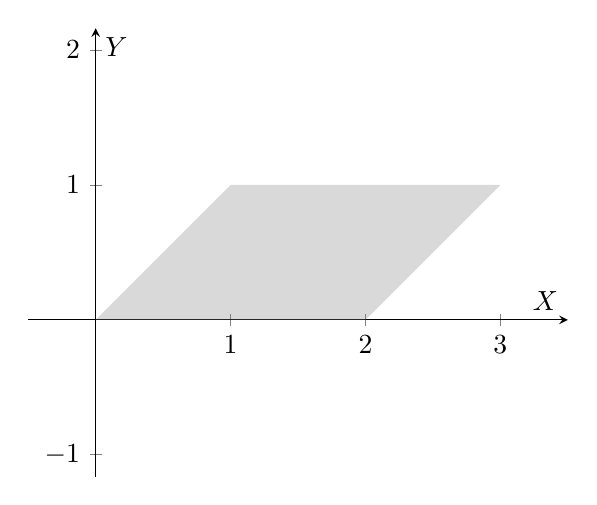
\begin{tikzpicture}
            \begin{axis}[
                axis lines = center,
                xlabel = $X$,
                ylabel = $Y$,
                xmin=-0.5, xmax=3.5,
                ymin=-0.5, ymax=1.5,
                axis equal,
                legend pos=outer north east,
            ]

            % Paralelogramo
            \addplot[fill=gray, fill opacity=0.3, draw=none, forget plot] coordinates {(0,0) (2,0) (3,1) (1,1)};

            \end{axis}
        \end{tikzpicture}
    \end{figure}

    Notemos por $P$ al paralelogramo. Tenemos que la función de densidad conjunta es:
    \begin{equation*}
        f_{(X,Y)}(x, y) = \begin{cases}
            k, & (x, y)\in P\\
            0, & \text{en otro caso}
        \end{cases}
    \end{equation*}
    Para calcular $k$, tenemos que:
    \begin{equation*}
        1=\int_P f_{(X,Y)} = \int_P k = k\lm(P) = k\cdot 2\cdot 1 = 2k \Longrightarrow k = \dfrac{1}{2}
    \end{equation*}

    Calculamos en primer lugar las marginales. Para $x\in [0,3]$, tenemos que:
    \begin{itemize}
        \item Si $x\in [0,1]$, tenemos que:
        \begin{equation*}
            f_X(x) = \int_{0}^{x} \dfrac{1}{2} \ dy = \dfrac{x}{2}
        \end{equation*}

        \item Si $x\in [1,2]$, tenemos que:
        \begin{equation*}
            f_X(x) = \int_{0}^{1} \dfrac{1}{2} \ dy = \dfrac{1}{2}
        \end{equation*}

        \item Si $x\in [2,3]$, tenemos que:
        \begin{equation*}
            f_X(x) = \int_{x-2}^{1} \dfrac{1}{2} \ dy = \dfrac{1}{2}(1-x+2)
            = \frac{3-x}{2}
        \end{equation*}
    \end{itemize}
    Por tanto, tenemos que:
    \begin{equation*}
        f_X(x) = \begin{cases}
            \nicefrac{x}{2}, & x\in [0,1]\\
            \nicefrac{1}{2}, & x\in [1,2]\\
            \frac{3-x}{2}, & x\in [2,3]\\
            0, & \text{en otro caso}
        \end{cases}
    \end{equation*}

    Para $y\in [0,1]$, tenemos que:
    \begin{equation*}
        f_Y(y) = \int_{y}^{y+2} \dfrac{1}{2} \ dx = \dfrac{1}{2}(y+2-y) = 1
    \end{equation*}

    Calculamos ahora las condicionadas. Dado $y^*\in [0,1]$, tenemos que:
    \begin{equation*}
        f_{X\mid Y=y^*}(x) = \dfrac{f_{(X,Y)}(x, y^*)}{f_Y(y^*)} = \dfrac{\nicefrac{1}{2}}{1} = \dfrac{1}{2} \qquad \forall x\in [0,3]
    \end{equation*}

    Respecto a la condicionada de $Y$ dado $X=x^*$, distinguimos en función de $x^*$:
    \begin{equation*}
        f_{Y\mid X=x^*}(y) = \dfrac{f_{(X,Y)}(x^*, y)}{f_X(x^*)} = \begin{cases}
            \nicefrac{1}{x^*}, & x^*\in [0,1],~y\in [0,x^*]\\
            \nicefrac{1}{2}, & x^*\in [1,2],~y\in [0,1]\\
            \frac{1}{3-x^*}, & x^*\in [2,3],~y\in [x^*-2,1]
        \end{cases}
    \end{equation*}

    Tenemos que calcular los siguientes errores cuadráticos medios:
    \begin{align*}
        \text{ECM}(\wh{X}(Y)) &= E[\Var[X\mid Y]]\\
        \text{ECM}(\wh{Y}(X)) &= E[\Var[Y\mid X]]
    \end{align*}

    Para calcular $E[\Var[X\mid Y]]$, tenemos que:
    \begin{align*}
        E[X\mid Y=y] &= \int_{y}^{y+2} x\cdot \dfrac{1}{2} \ dx
        = \dfrac{1}{2}\left[\dfrac{x^2}{2}\right]_{y}^{y+2}
        = \dfrac{1}{2}\left(\dfrac{(y+2)^2}{2}-\dfrac{y^2}{2}\right)
        = \dfrac{4y-4}{4} = y-1\\
        E[X^2\mid Y=y] &= \int_{y}^{y+2} x^2\cdot \dfrac{1}{2} \ dx
        = \dfrac{1}{2}\left[\dfrac{x^3}{3}\right]_{y}^{y+2}
        = \dfrac{1}{2}\left(\dfrac{(y+2)^3}{3}-\dfrac{y^3}{3}\right)
        = \dfrac{6y^2+12y+8}{6} =\\&= y^2+2y+\nicefrac{4}{3}\\
        \Var[X\mid Y=y] &= E[X^2\mid Y=y]-E[X\mid Y=y]^2
        = y^2+2y+\dfrac{4}{3}-(y-1)^2
        =\\&= y^2+2y+\nicefrac{4}{3}-y^2+2y-1
        = 4y+\nicefrac{1}{3}\\
        E[Y] &= \int_{0}^{1} y \ dy = \left[\dfrac{y^2}{2}\right]_{0}^{1} = \dfrac{1}{2}\\
        E[\Var[X\mid Y]] &= E\left[4Y+\dfrac{1}{3}\right] = 4E[Y]+\dfrac{1}{3} = 2+\dfrac{1}{3} = \dfrac{7}{3}
    \end{align*}

    % // TODO: Continuar para la otra
\end{ejercicio}

\begin{ejercicio}
    Sea $(X,Y)$ un vector aleatorio con rectas de regresión
    \begin{equation*}
        x+4y = 1 \qquad x+5y = 2
    \end{equation*}
    \begin{enumerate}
        \item ¿Cuál es la recta de regresión de $Y$ sobre $X$?
        
        Suponemos que la recta de regresión de $Y$ sobre $X$ es $x+4y=1$. Por tanto, tenemos que:
        \begin{equation*}
            y=\wh{Y}(x) = \dfrac{1}{4}-\dfrac{x}{4} = E[Y] + \dfrac{\Cov[X,Y]}{\Var[X]}\left(x-E[X]\right)
            \Longrightarrow
            \dfrac{\Cov[X,Y]}{\Var[X]} = -\dfrac{1}{4}
        \end{equation*}

        Por otro lado, tenemos que la recta de regresión de $X$ sobre $Y$ es $x+5y=2$. Por tanto, tenemos que:
        \begin{equation*}
            x=\wh{X}(y) = 2-5y = E[X] + \dfrac{\Cov[X,Y]}{\Var[Y]}\left(y-E[Y]\right)
            \Longrightarrow
            \dfrac{\Cov[X,Y]}{\Var[Y]} = -5
        \end{equation*}

        Por tanto, el coeficiente de determinación lineal es:
        \begin{equation*}
            \rho_{X/Y}^2 = \dfrac{\Cov[X,Y]^2}{\Var[X]\Var[Y]} = -\dfrac{1}{4}\cdot (-5) = \dfrac{5}{4}>1
        \end{equation*}

        Esto es un absurdo, luego nuestra suposición era errónea. La recta de regresión de $Y$ sobre $X$ es $x+5y=2$ y la de $X$ sobre $Y$ es $x+4y=1$.
        
        
        \item Calcular el coeficiente de correlación lineal y la proporción de varianza de cada variable que queda explicada por la regresión lineal.
        
        Como la recta de regresión de $Y$ sobre $X$ es $x+5y=2$, tenemos que:
        \begin{equation*}
            y=\wh{Y}(x) = \dfrac{2-x}{5} = E[Y] + \dfrac{\Cov[X,Y]}{\Var[X]}\left(x-E[X]\right)
            \Longrightarrow
            \dfrac{\Cov[X,Y]}{\Var[X]} = -\dfrac{1}{5}
        \end{equation*}

        Por otro lado, como la recta de regresión de $X$ sobre $Y$ es $x+4y=1$, tenemos que:
        \begin{equation*}
            x=\wh{X}(y) = 1-4y = E[X] + \dfrac{\Cov[X,Y]}{\Var[Y]}\left(y-E[Y]\right)
            \Longrightarrow
            \dfrac{\Cov[X,Y]}{\Var[Y]} = -4
        \end{equation*}

        Por tanto, el coeficiente de determinación lineal es:
        \begin{equation*}
            \rho_{X/Y}^2 = \dfrac{\Cov[X,Y]^2}{\Var[X]\Var[Y]} = -\dfrac{1}{5}\cdot (-4) = \dfrac{4}{5} = 0.8
        \end{equation*}

        Por tanto, la proporción de varianza de cada variable que queda explicada por la regresión lineal es un $80\%$. Además, como la covarianza es negativa, el coeficiente de correlación lineal es:
        \begin{equation*}
            \rho_{X/Y} = -\sqrt{\rho_{X/Y}^2} = -\sqrt{\dfrac{4}{5}} = -\dfrac{2\sqrt{5}}{5}
        \end{equation*}

        \item Calcular las medias de ambas variables.
        
        De la forma de las rectas de regresión, planteamos el siguiente sistema:
        \begin{equation*}
            \begin{cases}
                E[Y] +\nicefrac{1}{5}E[X] = \nicefrac{2}{5}\\
                E[X] +4E[Y] = 1
            \end{cases}
        \end{equation*}

        Resolviendo el sistema, llegamos a que:
        \begin{equation*}
            E[X]=-3 \qquad E[Y]=1
        \end{equation*}
    \end{enumerate}
\end{ejercicio}